\documentclass[border=8pt]{standalone}
\usepackage[T1]{fontenc}\usepackage{helvet}\renewcommand{\familydefault}{\sfdefault}
\usepackage{tikz}\usetikzlibrary{arrows.meta, positioning, calc, backgrounds}
\definecolor{ink}{HTML}{1a1916}
\definecolor{inktwo}{HTML}{3a3a35}
\definecolor{inkthree}{HTML}{6a6862}
\definecolor{rule}{HTML}{b8b09a}
\definecolor{amber}{HTML}{a8730a}
\definecolor{red}{HTML}{c8261a}
\definecolor{paper}{HTML}{f0eee5}
\definecolor{slab}{HTML}{d8d4c6}
\tikzset{
  >={Stealth[length=2.2mm]},
  wire/.style={line width=0.8pt, ink},
  modwire/.style={line width=0.6pt, dashed, ink},
  tastewire/.style={line width=0.6pt, dashed, amber},
  gatewire/.style={line width=0.6pt, dotted, ink},
  block/.style={rectangle, draw=ink, line width=0.9pt, fill=slab, minimum width=3.0cm, minimum height=1.9cm, inner sep=0pt},
  perf/.style={rectangle, draw=ink, line width=0.7pt, minimum width=3.0cm, minimum height=0.7cm, inner sep=2pt, font=\footnotesize, text=ink},
  title/.style={font=\scriptsize\bfseries, text=ink, anchor=north, inner sep=2pt},
  jack/.style={circle, draw=ink, fill=paper, line width=0.5pt, minimum size=3.2pt, inner sep=0pt},
  plabel/.style={font=\tiny, text=inktwo, anchor=west, inner sep=1pt},
  olabel/.style={font=\tiny, text=inktwo, anchor=east, inner sep=1pt},
  settings/.style={font=\scriptsize, text=ink, align=left, anchor=north west, inner sep=1pt, text width=2.9cm},
}
\begin{document}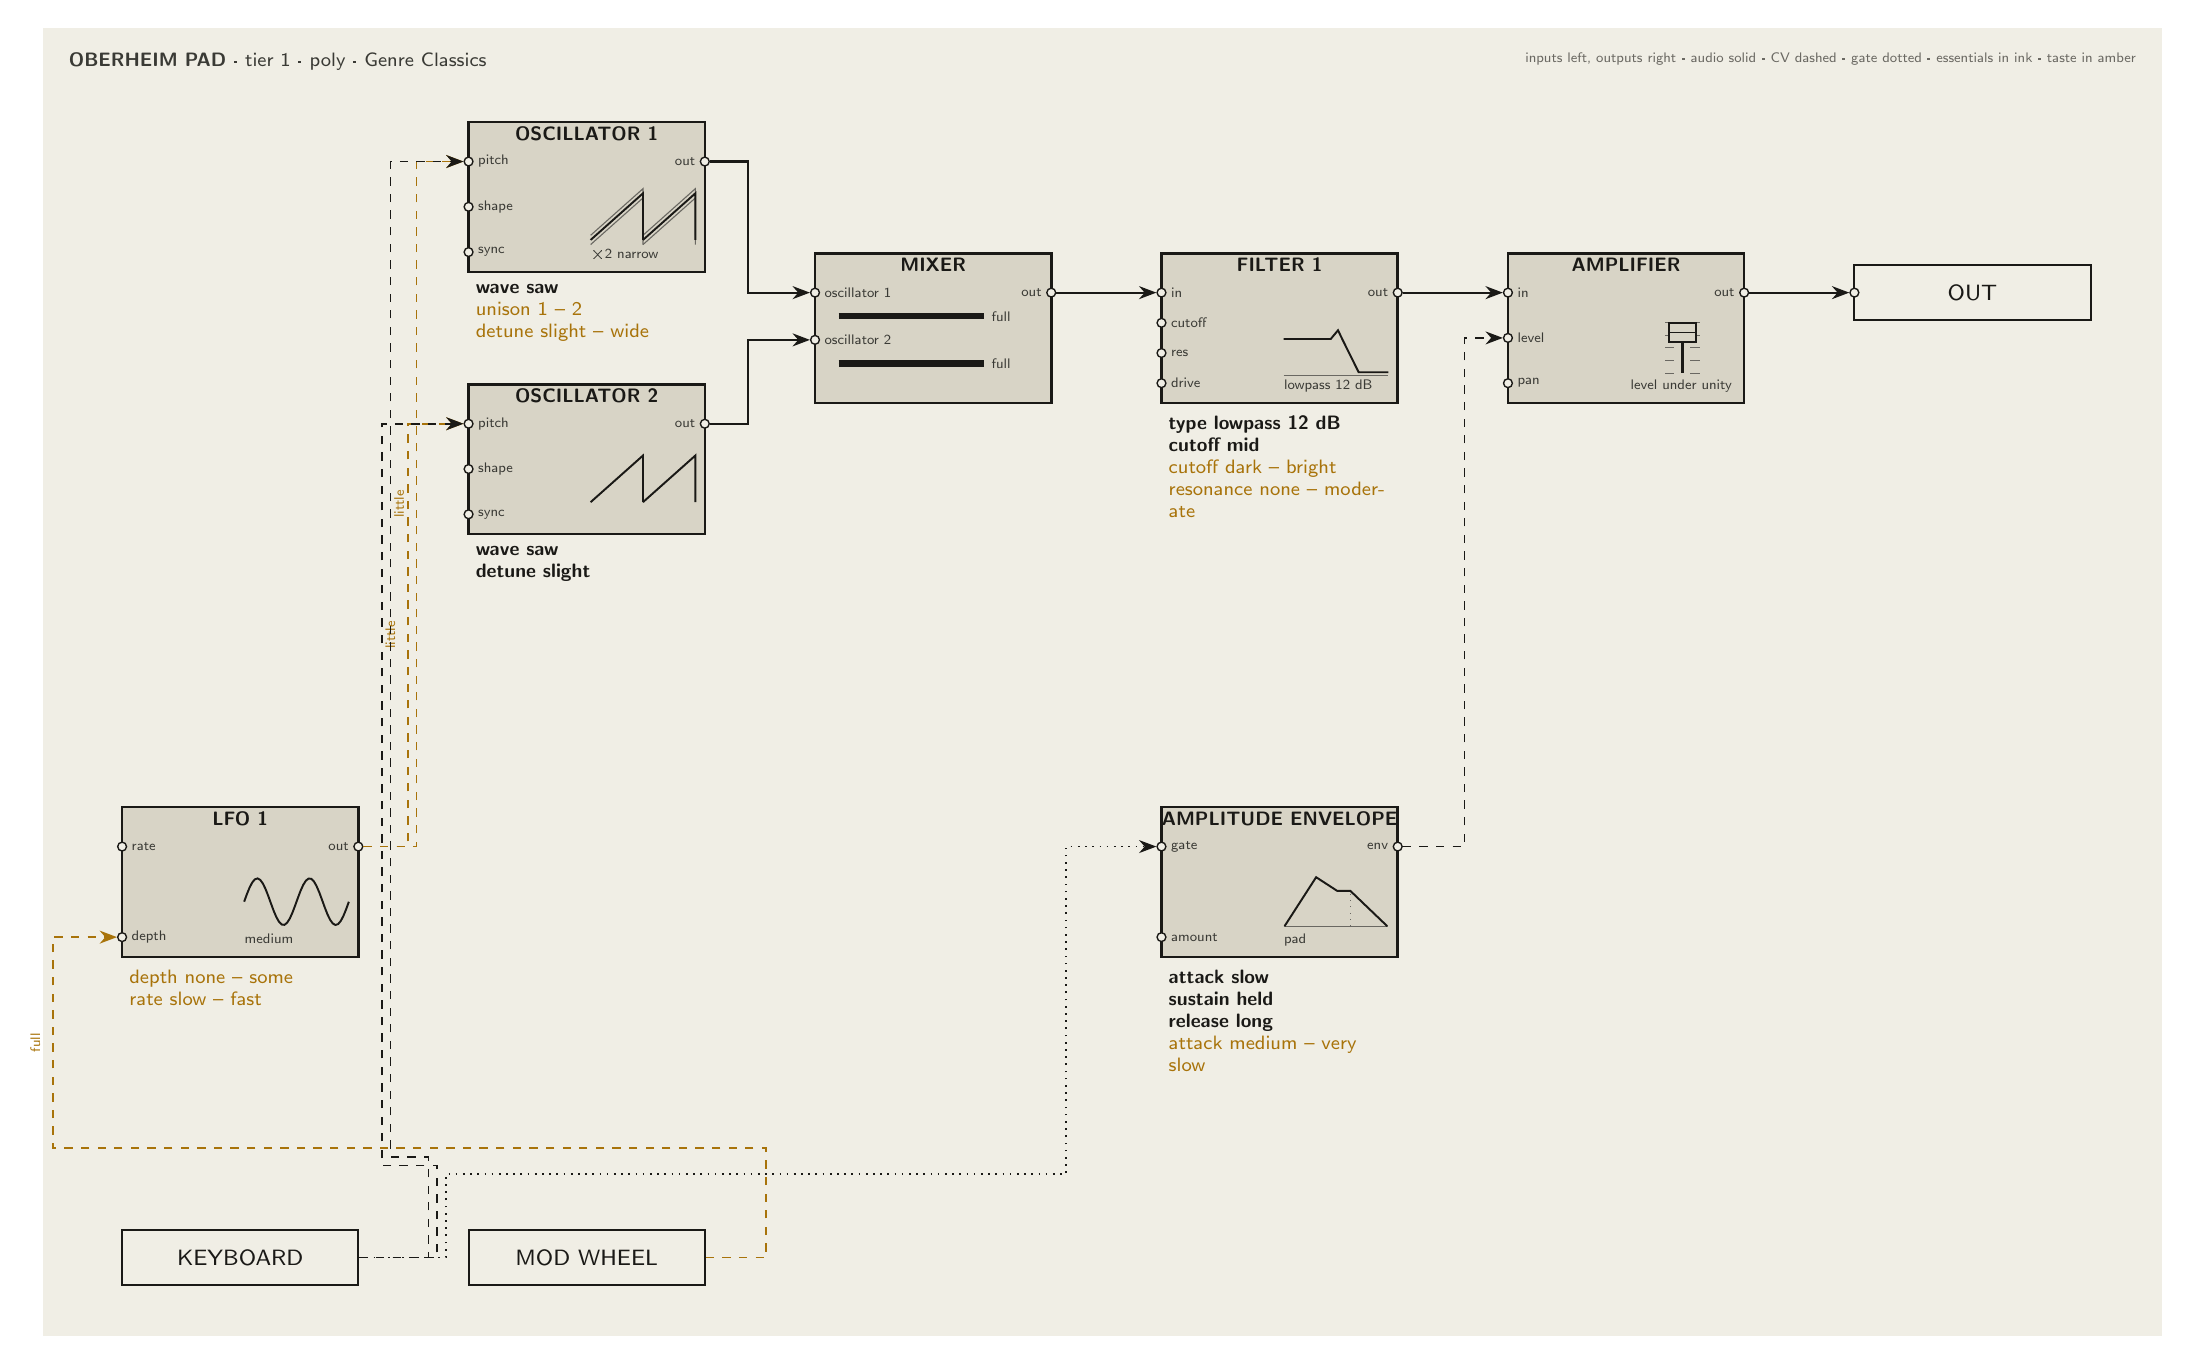
\begin{tikzpicture}
\begin{scope}[on background layer]\fill[paper] (-2.5,-12.805) rectangle (24.4,3.8150000000000004);\end{scope}
\node[block, minimum height=1.9cm] (osc1) at (4.4,1.665) {};
\node[title] at (osc1.north) {OSCILLATOR 1};
\node[jack] (osc1-pitch) at (2.9000000000000004,2.115) {};
\node[plabel] at (2.9800000000000004,2.115) {pitch};
\node[jack] (osc1-shape) at (2.9000000000000004,1.5400000000000003) {};
\node[plabel] at (2.9800000000000004,1.5400000000000003) {shape};
\node[jack] (osc1-sync) at (2.9000000000000004,0.9650000000000003) {};
\node[plabel] at (2.9800000000000004,0.9650000000000003) {sync};
\node[jack] (osc1-out) at (5.9,2.115) {};
\node[olabel] at (5.82,2.115) {out};
\begin{scope}
\draw[inkthree, line width=0.4pt] (4.450,1.178) -- (5.115,1.770) -- (5.115,1.178);
\draw[inkthree, line width=0.4pt] (5.115,1.178) -- (5.780,1.770) -- (5.780,1.178);
\draw[inkthree, line width=0.4pt] (4.450,1.060) -- (5.115,1.652) -- (5.115,1.060);
\draw[inkthree, line width=0.4pt] (5.115,1.060) -- (5.780,1.652) -- (5.780,1.060);
\draw[ink, line width=0.7pt] (4.450,1.119) -- (5.115,1.711) -- (5.115,1.119);
\draw[ink, line width=0.7pt] (5.115,1.119) -- (5.780,1.711) -- (5.780,1.119);
\node[font=\tiny, text=inktwo, anchor=north west, inner sep=0pt] at (4.450,1.015) {×2 narrow};
\end{scope}
\node[settings] at (2.95,0.5950000000000001) {\textbf{wave saw} \\ \textcolor{amber}{unison 1 -- 2} \\ \textcolor{amber}{detune slight -- wide}};
\node[block, minimum height=1.9cm] (osc2) at (4.4,-1.665) {};
\node[title] at (osc2.north) {OSCILLATOR 2};
\node[jack] (osc2-pitch) at (2.9000000000000004,-1.215) {};
\node[plabel] at (2.9800000000000004,-1.215) {pitch};
\node[jack] (osc2-shape) at (2.9000000000000004,-1.79) {};
\node[plabel] at (2.9800000000000004,-1.79) {shape};
\node[jack] (osc2-sync) at (2.9000000000000004,-2.365) {};
\node[plabel] at (2.9800000000000004,-2.365) {sync};
\node[jack] (osc2-out) at (5.9,-1.215) {};
\node[olabel] at (5.82,-1.215) {out};
\begin{scope}
\draw[ink, line width=0.7pt] (4.450,-2.211) -- (5.115,-1.619) -- (5.115,-2.211);
\draw[ink, line width=0.7pt] (5.115,-2.211) -- (5.780,-1.619) -- (5.780,-2.211);
\end{scope}
\node[settings] at (2.95,-2.7350000000000003) {\textbf{wave saw} \\ \textbf{detune slight}};
\node[block, minimum height=1.9cm] (mix) at (8.8,0.0) {};
\node[title] at (mix.north) {MIXER};
\node[jack] (mix-osc1) at (7.300000000000001,0.44999999999999996) {};
\node[plabel] at (7.380000000000001,0.44999999999999996) {oscillator 1};
\draw[inkthree, line width=0.3pt] (7.600,0.150) -- (9.450,0.150);
\draw[ink, line width=2.2pt] (7.600,0.150) -- (9.450,0.150);
\node[font=\tiny, text=inktwo, anchor=west, inner sep=1pt] at (9.500,0.150) {full};
\node[jack] (mix-osc2) at (7.300000000000001,-0.15000000000000002) {};
\node[plabel] at (7.380000000000001,-0.15000000000000002) {oscillator 2};
\draw[inkthree, line width=0.3pt] (7.600,-0.450) -- (9.450,-0.450);
\draw[ink, line width=2.2pt] (7.600,-0.450) -- (9.450,-0.450);
\node[font=\tiny, text=inktwo, anchor=west, inner sep=1pt] at (9.500,-0.450) {full};
\node[jack] (mix-out) at (10.3,0.44999999999999996) {};
\node[olabel] at (10.22,0.44999999999999996) {out};
\node[block, minimum height=1.9cm] (filter1) at (13.200000000000001,0.0) {};
\node[title] at (filter1.north) {FILTER 1};
\node[jack] (filter1-in) at (11.700000000000001,0.44999999999999996) {};
\node[plabel] at (11.780000000000001,0.44999999999999996) {in};
\node[jack] (filter1-cutoff) at (11.700000000000001,0.06666666666666665) {};
\node[plabel] at (11.780000000000001,0.06666666666666665) {cutoff};
\node[jack] (filter1-res) at (11.700000000000001,-0.31666666666666665) {};
\node[plabel] at (11.780000000000001,-0.31666666666666665) {res};
\node[jack] (filter1-drive) at (11.700000000000001,-0.7) {};
\node[plabel] at (11.780000000000001,-0.7) {drive};
\node[jack] (filter1-out) at (14.700000000000001,0.44999999999999996) {};
\node[olabel] at (14.620000000000001,0.44999999999999996) {out};
\begin{scope}
\draw[inkthree, line width=0.3pt] (13.250,-0.605) -- (14.580,-0.605);
\draw[ink, line width=0.7pt] (13.250,-0.139) -- (13.849,-0.139) -- (13.942,-0.028) -- (13.995,-0.139) -- (14.204,-0.561) -- (14.580,-0.561);
\node[font=\tiny, text=inktwo, anchor=north west, inner sep=0pt] at (13.250,-0.650) {lowpass 12 dB};
\end{scope}
\node[settings] at (11.750000000000002,-1.0699999999999998) {\textbf{type lowpass 12 dB} \\ \textbf{cutoff mid} \\ \textcolor{amber}{cutoff dark -- bright} \\ \textcolor{amber}{resonance none -- moderate}};
\node[block, minimum height=1.9cm] (amp) at (17.6,0.0) {};
\node[title] at (amp.north) {AMPLIFIER};
\node[jack] (amp-in) at (16.1,0.44999999999999996) {};
\node[plabel] at (16.18,0.44999999999999996) {in};
\node[jack] (amp-level) at (16.1,-0.125) {};
\node[plabel] at (16.18,-0.125) {level};
\node[jack] (amp-pan) at (16.1,-0.7) {};
\node[plabel] at (16.18,-0.7) {pan};
\node[jack] (amp-out) at (19.1,0.44999999999999996) {};
\node[olabel] at (19.020000000000003,0.44999999999999996) {out};
\begin{scope}
\draw[ink, line width=1.2pt] (18.315,-0.570) -- (18.315,0.070);
\draw[inkthree, line width=0.3pt] (18.095,-0.570) -- (18.215,-0.570) (18.415,-0.570) -- (18.535,-0.570);
\draw[inkthree, line width=0.3pt] (18.095,-0.410) -- (18.215,-0.410) (18.415,-0.410) -- (18.535,-0.410);
\draw[inkthree, line width=0.3pt] (18.095,-0.250) -- (18.215,-0.250) (18.415,-0.250) -- (18.535,-0.250);
\draw[inkthree, line width=0.3pt] (18.095,-0.090) -- (18.215,-0.090) (18.415,-0.090) -- (18.535,-0.090);
\draw[inkthree, line width=0.3pt] (18.095,0.070) -- (18.215,0.070) (18.415,0.070) -- (18.535,0.070);
\fill[slab, draw=ink, line width=0.6pt] (18.145,-0.178) rectangle (18.485,0.062);
\draw[ink, line width=0.5pt] (18.145,-0.058) -- (18.485,-0.058);
\node[font=\tiny, text=inktwo, anchor=north west, inner sep=0pt] at (17.650,-0.650) {level under unity};
\end{scope}
\node[block, minimum height=1.9cm] (lfo1) at (0.0,-7.035000000000001) {};
\node[title] at (lfo1.north) {LFO 1};
\node[jack] (lfo1-rate) at (-1.5,-6.585000000000001) {};
\node[plabel] at (-1.42,-6.585000000000001) {rate};
\node[jack] (lfo1-depth) at (-1.5,-7.735000000000001) {};
\node[plabel] at (-1.42,-7.735000000000001) {depth};
\node[jack] (lfo1-out) at (1.5,-6.585000000000001) {};
\node[olabel] at (1.42,-6.585000000000001) {out};
\begin{scope}
\draw[ink, line width=0.7pt] plot[domain=0:1, samples=40, variable=\u] ({0.050+\u*1.330},{-7.655+(0.740)*(0.5+0.4*sin(360*\u*2))});
\node[font=\tiny, text=inktwo, anchor=north west, inner sep=0pt] at (0.050,-7.685) {medium};
\end{scope}
\node[settings] at (-1.45,-8.105) {\textcolor{amber}{depth none -- some} \\ \textcolor{amber}{rate slow -- fast}};
\node[block, minimum height=1.9cm] (aenv) at (13.200000000000001,-7.035000000000001) {};
\node[title] at (aenv.north) {AMPLITUDE ENVELOPE};
\node[jack] (aenv-gate) at (11.700000000000001,-6.585000000000001) {};
\node[plabel] at (11.780000000000001,-6.585000000000001) {gate};
\node[jack] (aenv-amount) at (11.700000000000001,-7.735000000000001) {};
\node[plabel] at (11.780000000000001,-7.735000000000001) {amount};
\node[jack] (aenv-out) at (14.700000000000001,-6.585000000000001) {};
\node[olabel] at (14.620000000000001,-6.585000000000001) {env};
\begin{scope}
\draw[inkthree, line width=0.3pt] (13.250,-7.596) -- (14.580,-7.596);
\draw[ink, line width=0.7pt] (13.263,-7.596) -- (13.664,-6.974) -- (13.932,-7.148) -- (14.099,-7.148) -- (14.567,-7.596);
\draw[inkthree, line width=0.3pt, dotted] (14.099,-7.596) -- (14.099,-7.148);
\node[font=\tiny, text=inktwo, anchor=north west, inner sep=0pt] at (13.250,-7.685) {pad};
\end{scope}
\node[settings] at (11.750000000000002,-8.105) {\textbf{attack slow} \\ \textbf{sustain held} \\ \textbf{release long} \\ \textcolor{amber}{attack medium -- very slow}};
\node[perf] (key) at (0.0,-11.805) {KEYBOARD};
\node[perf] (wheel) at (4.4,-11.805) {MOD WHEEL};
\node[perf, fill=paper] (out) at (22.0,0.44999999999999996) {OUT}; \node[jack] (out-in) at (20.5,0.44999999999999996) {};
\draw[wire,->] (osc1-out) -- (6.45,2.115) |- (mix-osc1);
\draw[wire,->] (osc2-out) -- (6.45,-1.215) |- (mix-osc2);
\draw[wire,->] (mix-out) -- (filter1-in);
\draw[wire,->] (filter1-out) -- (amp-in);
\draw[wire,->] (amp-out) -- (out-in);
\draw[modwire,->] (aenv-out) -- (15.55,-6.585000000000001) -- (15.55,-0.125) -- (amp-level);
\draw[tastewire,->] (lfo1-out) -- (2.2400000000000007,-6.585000000000001) -- (2.2400000000000007,2.115) -- (osc1-pitch);
\node[font=\tiny, text=amber, anchor=south, inner sep=1pt, rotate=90] at (2.1200000000000006,-2.2350000000000003) {little};
\draw[tastewire,->] (lfo1-out) -- (2.1300000000000003,-6.585000000000001) -- (2.1300000000000003,-1.215) -- (osc2-pitch);
\node[font=\tiny, text=amber, anchor=south, inner sep=1pt, rotate=90] at (2.0100000000000002,-3.9000000000000004) {little};
\draw[tastewire,->] (wheel.east) -- (6.680000000000001,-11.805) -- (6.680000000000001,-10.415000000000001) -- (-2.38,-10.415000000000001) -- (-2.38,-7.735000000000001) -- (lfo1-depth);
\node[font=\tiny, text=amber, anchor=south, inner sep=1pt, rotate=90] at (-2.5,-9.075000000000001) {full};
\draw[modwire,->] (key.east) -- (2.39,-11.805) -- (2.39,-10.525) -- (1.9100000000000006,-10.525) -- (1.9100000000000006,2.115) -- (osc1-pitch);
\draw[modwire,->] (key.east) -- (2.5,-11.805) -- (2.5,-10.635000000000002) -- (1.8000000000000005,-10.635000000000002) -- (1.8000000000000005,-1.215) -- (osc2-pitch);
\draw[gatewire,->] (key.east) -- (2.61,-11.805) -- (2.61,-10.745000000000001) -- (10.49,-10.745000000000001) -- (10.49,-6.585000000000001) -- (aenv-gate);
\node[anchor=north west, font=\scriptsize, text=inktwo] at (-2.3,3.615) {\textbf{OBERHEIM PAD} · tier 1 · poly · Genre Classics};
\node[anchor=north east, font=\tiny, text=inkthree] at (24.2,3.615) {inputs left, outputs right · audio solid · CV dashed · gate dotted · essentials in ink · taste in amber};
\end{tikzpicture}\end{document}
